\documentclass[12pt]{article}
\usepackage[2120943]{easymcm}
\usepackage{mathptmx}
\usepackage{float}
\usepackage{subfigure}

\problem{A}
\title{Analysis and Prediction of Fungi Decomposition Process}

\begin{document}

	\begin{abstract}
		Fungi play an indespensable role in the carbon cycle of our ecosystems. They free the trapped carbon in the debri of living creatures out into the cycle through metabolism. Environment for fungi's well-living is delicate. Any turbulence of temoerature, humidity, and the competition from within the populations would bring pressure to the fungal reproducction.
		
		First of all, we assume that the only resources, the woody fibres, are infinite, thus build a mathematical model using N-species CLV equations to describe the growth of fungi populationj without limit of population capacity. To build the model we assume some of the paramaters of the growth of fungi. The model demostrates that.
		
		In the second step, we take the limitation of woody fibres into account, and adjust Model1 to fit the new population model. The new model showa that 123.

		
		
		In addition, we test the minggandu and robustness\\
		\vspace{5pt}
		\textbf{Keywords}:
	\end{abstract}
	
	\maketitle
	\tableofcontents
	\section{Introduction}
	\subsection{Problem Background}
	There are many kinds of fungi on the earth. They are the primary decomposers of organic material in terrestrial ecosystems. Because of that, fungi are a functionally critical component of terrestrial ecosystems. Their decompose ability varys under different environment conditions and different species. To be more specific, environment conditions mainly refers to temperature and moisture and different species represents different traits like moisture tolerance, temperature tolerance, competitive rank and so on.
	\subsection{Restatement of the Problem}
	\begin{itemize}
		\item Build a mathematical model to simulate degradation process.
		\item Incoporate the interactions between different species to the previous model.
		\item Examine the sensitivity to rapid fluctuations in the environment.
		\item The advantage and disadvantage for each species under different environment
		\item Examine the importance of biodiversity
	\end{itemize}
	
	\subsection{Our Work}
	The topic requires us to simulate the growth of fungi community and then consider their impact on the plant material. Our work mainly includes the following:
	\begin{itemize}
		\item Based on the Competitive Lotka–Volterra equations and the data of fungi’s growth rate with respect to temperature and moisture, a population growth model is established.
		\item Consider the impact of plant material to fungi community to build the decomposition model.
		\item Change the climate and make rapid fluctuations to the model to discuss the outcome.
	\end{itemize}	
	\section{Model Preperation}
	\subsection{Assumptions}
	\begin{itemize}
		\item Fungi community is applied to Competitive Lotka-Volterra equations
		\item Research data is accurate
		\item The parameters estimated from the data, which were generated from standardized experiment, are fungi's inherent traits
	\end{itemize}
	\subsection{Notations}
	Important notations used in this paper are listed in Table \ref{tb:notation}
	\begin{table}[H]
		\begin{center}
		\caption{Notations}
		\begin{tabular}{ccc}
			\toprule
			Symbol& Definition &Unit\\
			\midrule
			$T$&Temperature in Celcius&$^{\circ}\text{C}$\\
			\specialrule{0em}{1pt}{1pt}
			$M$&Moisture&MPa\\  
			\specialrule{0em}{1pt}{1pt}
			$n_i$&Fungi's Competitive Rank&$n \text{ is scaled to } [0,1]$\\
			\specialrule{0em}{1pt}{1pt}
			$v_{\text{extension}}$&Fungi's Extension Rate&$\text{mm/day}$\\
			\specialrule{0em}{1pt}{1pt}
			$\rho_{\textrm{hyphae}}$&Hyphae Density & $\mu \text g/ \text{cm}^2$ \\
			\specialrule{0em}{1pt}{1pt}
			$S_i$ &Fungi's Popluation Size& $\mu \text g$\\ 
			\specialrule{0em}{1pt}{1pt}
			$K_i$ & Bioligical Capacity& $\mu \text g$\\
			\specialrule{0em}{1pt}{1pt}
			$M_{\text{woody}}$ & Weight of the Woody&$\mu \text g$\\
			\bottomrule
		\end{tabular}\label{tb:notation}
		\end{center}
	\end{table}		
	\subsection{Data Collection}
	The data we use mainly include several kinds of fungi's growth rate with temperature and moisture and their inherent traits. The data sources are summarized in Table \ref{tb:data}.
	\begin{table}[!htbp]
	\begin{center}
		\caption{Data Sources}
		\begin{tabular}{cll}
			\toprule
			\multicolumn{1}{m{5cm}}{\centering Data}
			&\multicolumn{1}{m{5cm}}{\centering Source}\\
			\midrule
			Fungi Variable and Description & https://www.pnas.org/content/pnas/117/21/11551.full.pdf\\
			Fungal\_trait\_data.csv&https://github.com/dsmaynard/fungal\_biogeography\\
			Fungi\_moisture\_curves.csv& https://github.com/dsmaynard/fungal\_biogeography\\
			Fungi\_temperature\_curves.csv& https://github.com/dsmaynard/fungal\_biogeography\\
			\bottomrule
		\end{tabular}\label{tb:data}
	\end{center}	
	\end{table}
	\section{Model 1:Fungi Population Prediction Model}
\subsection{Competitive Lotka-Volterra equations}
	Our final goal of modeling is to simulate the degradation of plant material by fungi. Therefore, at first we should resolve how will fungi community evolve under given environment conditions. In our model, there are competitions between different fungi species rather than predator-prey relationship. And all these species compete for common resource, plant material. Thus, the Competitive Lotka-Volterra Equations (CLV) is  well adopted to depict fungi population dynamics. 

	The N-species CLV equations are: 
	\begin{align}\label{CLV}
		\frac{\textrm d S_i}{\textrm d t}=r_iS_i(1-\frac{\sum_{j=1}^N\alpha_{ij}S_j}{K_i})
	\end{align}  

	where $S_i(t)$ is the size of the $i$-th population at a given time, $N$ is the total number interacting species, $r_i$ is inherent per-capita growth rate of $i$-th species, $\alpha_{ij}$ represents the effect species j has on the population of species i and $K_i$ is the carrying capacity of $i$-th species.


 
\subsection{Parameter Estimation and Definition of CLV Equations}
\subsubsection{Carrying Capacity: $K$}
	In a given patch of land,  the overall living space is fixed. Therefore, the carrying capacity of one species is proportional to its density:
	\begin{align}
		K_i \propto \rho_i
	\end{align}

	In our model there is no need to know the specific value of $K_i$, only the relative value matters.
	
\subsubsection{Inherent Per-capita Growth Rate: $r_i$}
	According to definition, we have:
	\begin{align}
		r_i \propto v_{\text{extension}}
	\end{align}
            
\subsubsection{Interaction Parameter: $\alpha_{ij}$}

	$\alpha_{ij}$ means the effect species j has on the population of species i. Here we use the competitive rank of fungi, which is accessible to us, to define the parameter. And two rules must be followed:
	\begin{itemize}
		\item All $\alpha$ values are positive
		\item $\alpha_{ij}=1$ when $i=j$
	\end{itemize}

	Therefore, we assume:
	\begin{align}
		\alpha_{ij}=\exp(1-\frac{n_i}{n_j})	
	\end{align}

	Where $n_i$ represents the competitive rank.(The bigger the $n_i$, the higher the ranking)


\subsection{Results}
3 kinds of fungi were selected.(Identifier:1,4,6. Refer to the appendix for detail traits) 

%-----------------------------------------------------------------
\iffalse
	6 kinds of fungi were selected. Refer to the appendix for details. 
	The computation was under such conditions:
 
	\begin{align}
    	T=22^{\circ}\text C,\ M=-0.5\text{MPa}\nonumber   
	\end{align}

	and the population evolution with time is shown in Figure \ref{fig:result1}

	\begin{figure}[H]
    	\centering
	    \includegraphics[width=.6\textwidth]{25_05.png}
    	\caption{The result of Model 1}\label{fig:result1}
    \end{figure}
 \fi
%-----------------------------------------------------------------  
\begin{figure}[htbp]
\centering
\subfigure[$T = 22^{\circ}\text C,\ M = -0.25\text{MPa}$]{
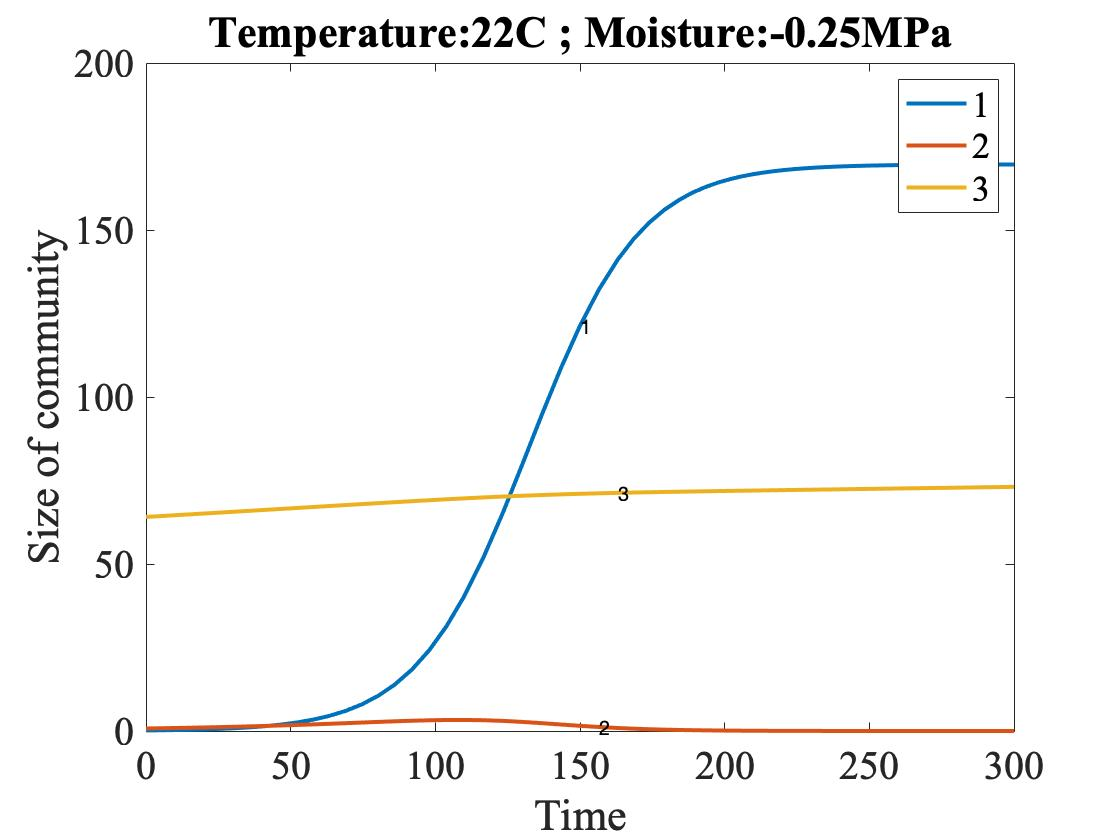
\includegraphics[width=6cm]{growth3_22_025.jpg}
%\caption{fig1}
}
\quad
\subfigure[$T = 25^{\circ}\text C,\ M = -0.5\text{MPa}$]{
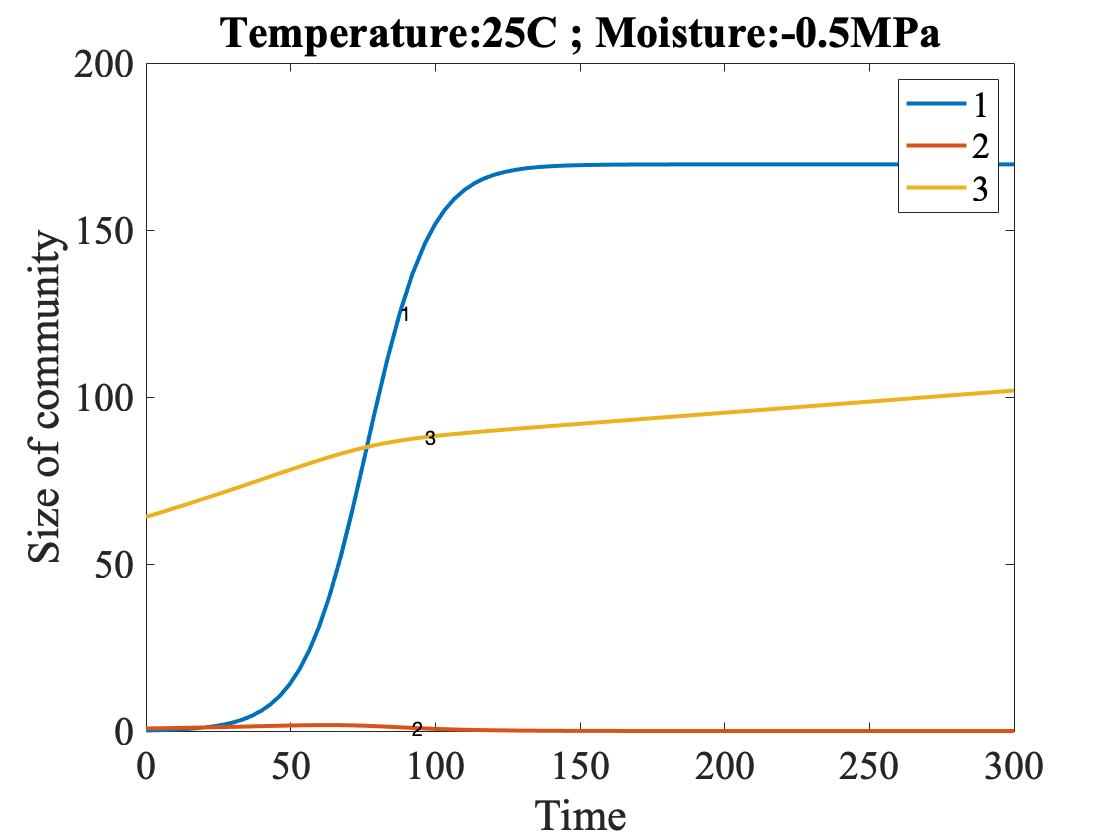
\includegraphics[width=6cm]{growth3_25_05.jpg}
}
\quad
\subfigure[$T = 25^{\circ}\text C,\ M = -2.5\text{MPa}$]{
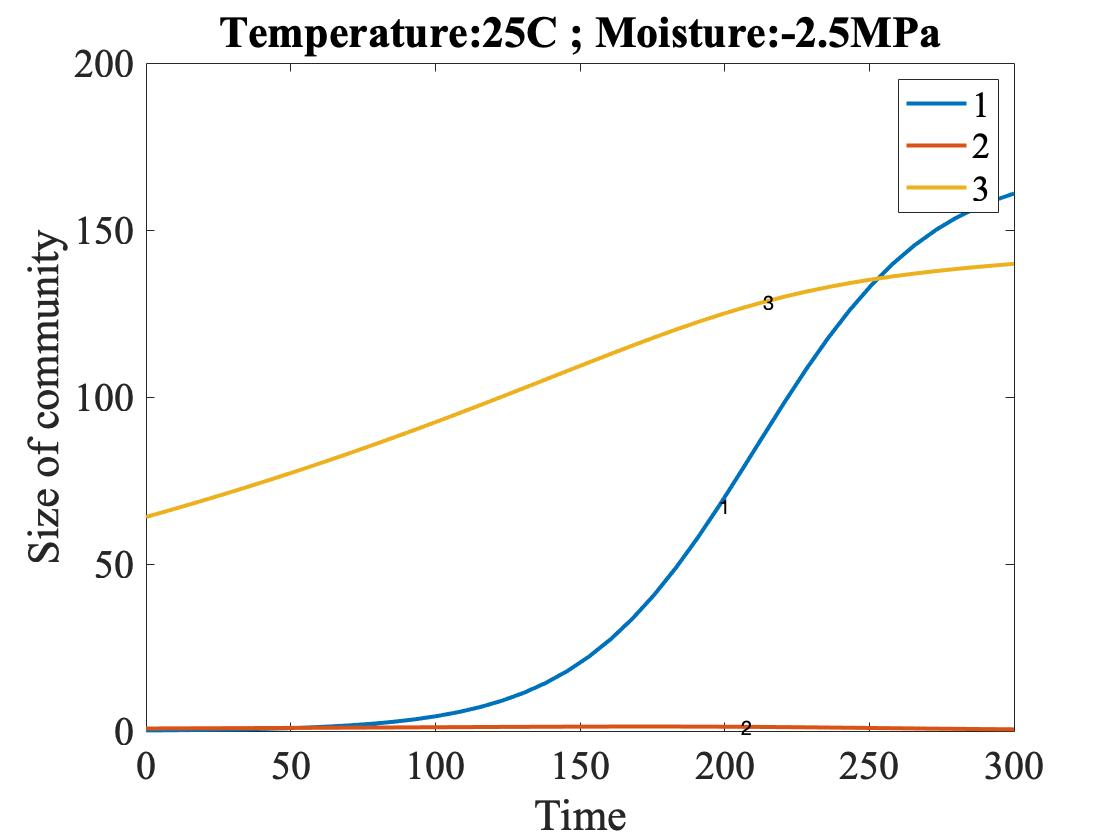
\includegraphics[width=6cm]{growth3_25_25.jpg}
}
\quad
\subfigure[$T = 33^{\circ}\text C,\ M = -0.5\text{MPa}$]{
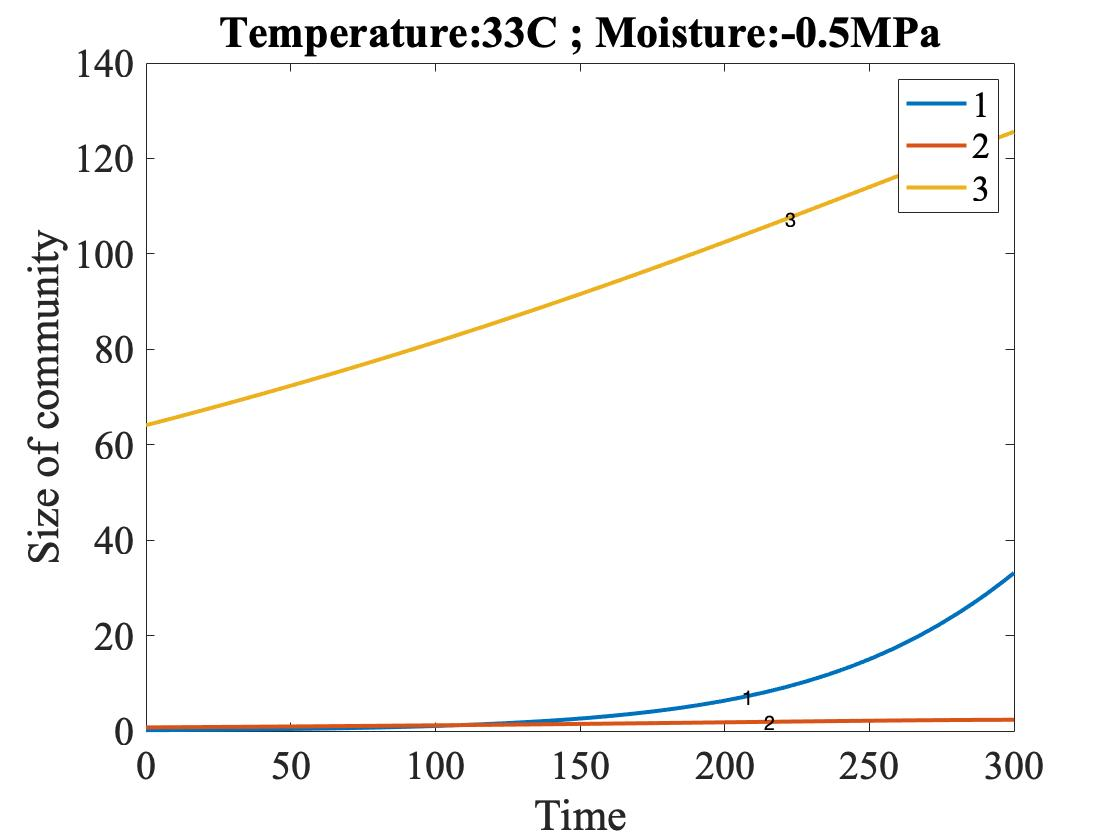
\includegraphics[width=6cm]{growth3_33_05.jpg}
}
\caption{Population Development}
\end{figure}



  
\subsection{Discussion}





















	\section{Model 2:Woody Fibres Decomposition Model}
	\subsection{Decomposition Equations}
	\subsection{Single Population}
		\subsubsection{Population Equation}
		According to the reference\cite{2}, the decomposition of wood confirms to the following model:

\begin{align}
    \frac{dS}{dt}=rS(1-S/K)\times M_{woody}\\
    \frac{dM_{woody}}{dt}=-\frac{r}{\epsilon}SM_{woody}
\end{align}
		\subsubsection{Results}
	\subsection{Multi Population}
		\subsubsection{Population Equation}
We assume that there are N kinds of different fungi, and the biomass of each kind of fungi is $S_i$. We only concern about the relative biomass of each kind of fungi, so we substitute $S_i$ with $x_i=S_i/K_i$.

We use the N-species Competitive Lotca-Voterra equations(\ref{CLV}).Using the substitution $x_i=S_i/K_i$, the equations are shown as follows:

\begin{align}
    \frac{dx_i}{dt}=r_i x_i  (1- \frac{\sum_{j=1}^{N}\alpha_{ij}x_jK_j}{K_i})
\end{align}
the parameters are listed as follows:
\begin{align}
    r_i&=\frac{v_{extension}}{R}\\
    K_i&=C\rho_i,C=const\\
    \alpha_{ij}&=\exp{1-\frac{n_i}{n_j}}
\end{align}

where $\epsilon=0.33$is efficiency, according to\cite{2}.

		\subsubsection{Results}


The results are shown in Figure \ref{fig:result}

\begin{figure}[H]
	\centering
	\includegraphics[width=.6\textwidth]{25_05_de.png}
	\caption{Decomposition Model}\label{fig:result}
\end{figure}

	\section{Test the Models}
 
\subsection{Sensitivity Analysis}
\subsection{Robustness}
	\input{Conclusion.tex}
	\section*{Referencese}
\begin{thebibliography}{99}

    \bibitem{2}Dang, Christian K. , et al. "Temperature oscillation coupled with fungal community shifts can modulate warming effects on litter decomposition." \emph{Ecology} 90.1(2009).
\end{thebibliography}
	\section*{Appendix}
\begin{table}[H]
		\begin{center}
		\caption{6 kinds of fungi trait}
		\begin{tabular}{ccccc}
			\toprule
			Number&Name &$n$ &Moisture Tolerance&$\rho_{\textrm{hyphae}}$\\
			\midrule
			1&Phlebia\_acerina\_DR60\_A8A&0.9459&1.28&0.27 \\
			\specialrule{0em}{1pt}{1pt}
			2&Tyromyces\_chioneus\_HHB11933\_B10F&0.6486&1.19&0.06\\
			\specialrule{0em}{1pt}{1pt}
			3&Hyphoderma\_setigerum\_HHB12156\_B3H&0.5675&1.19&0.09\\
			\specialrule{0em}{1pt}{1pt}
			4&Hyphodontia\_crustosa\_HHB13392\_B7B&0.3243&1.19&0.12\\
			\specialrule{0em}{1pt}{1pt}
			5&Armillaria\_sinapina\_PR9&0.1351&1.74&0.12\\
			\specialrule{0em}{1pt}{1pt}
			6&Armillaria\_gallica\_EL8\_A6F&0.02702&2.08&1.02\\
			\bottomrule
		\end{tabular}\label{tb:fungitrait}
		\end{center}
\end{table}		

	
\end{document}